\section{Graphing}

\subsection{Review problems}

\begin{enumerate}
\item Draw a coordinate plane and label the origin and the four quadrants.
\item Let $A = (3,1)$. Find the coordinates of each of the following:
\begin{enumerate}
\item the \href{https://en.wikipedia.org/wiki/Reflection_(mathematics)}{reflection} of $A$ across the $x$-axis
\item the reflection of $A$ across the $y$-axis
\item the reflection of $A$ across the line $y = x$
\item the \href{https://en.wikipedia.org/wiki/Rotation_(mathematics)}{rotation} of $A$ around the origin by $180^{\circ}$
\item the rotation of $A$ around the origin by $90^{\circ}$ counterclockwise
\item the rotation of $A$ around the point $(2,2)$ by $90^{\circ}$ clockwise
\end{enumerate}
\item Quadrilateral $ABCD$ is positioned in the coordinate plane so that its vertices have coordinates
\begin{equation*}
A = (5, 7);\quad B = (5, 6);\quad C = (3, 1);\quad D = (-4, -5).
\end{equation*}
Points $E, F, G, H$ are the midpoints of segments $\overline{AB}, \overline{BC}, \overline{CD}, \overline{DA}$, respectively.
\begin{enumerate}
\item Find the coordinates of $E$, $F$, $G$, and $H$.
\item Compute the midpoints of segments $\overline{EG}$ and $\overline{FH}$.
\end{enumerate}
To check your work, the two midpoints computed in part (b) should be the same. Doing this calculation in general (rather than with specific numbers) and finding that the midpoints of the diagonals of $EFGH$ coincide proves the following:
\begin{quote}
\textit{The midpoints of the sides of any quadrilateral form a parallelogram.}
\end{quote}
\item Maurine needs to get from $(2,3)$ to $(17,11)$.
\begin{enumerate}
\item If they take the shortest path possible, how much distance would they cover?
\item Suppose Maurine gets distracted while pondering the meaning of life and goes from $(2,3)$ to $(6,6)$, then to $(11, 18)$, then to $(17,10)$, and finally to $(17,11)$. What is the minimum distance Maurine can cover which is consistent with this information? 
\end{enumerate}
\item Which of the following expressions correctly finds the slope between the points $(-1,7)$ and $(3,-4)$? Circle all valid expressions.
\begin{equation*}
\frac{3 - (-1)}{-4 - 7}\qquad\frac{7 - (-4)}{-1 - 3}\qquad\frac{-4 - 7}{3 - (-1)}\qquad\frac{7 - (-4)}{3 - (-1)}\qquad\frac{-4 - 3}{7 - (-1)}
\end{equation*}
\item A line is given by the point-slope form
\begin{equation*}
y - 4 = \frac{1}{4}(x + 1).
\end{equation*}
\begin{enumerate}
\item Find the slope of the line and a point on the line.
\item Put the equation in slope-intercept form and find the $y$-intercept of the line.
\item Put the equation in standard form and find the $x$-intercept of the line.
\end{enumerate}
\item \begin{enumerate}
\item Of the equations
\begin{equation*}
5x + 4y = 35;\quad (x + 4)^2 + (y - 1)^2 = 10;\quad x^2 + xy + y^2 = 49;\quad x - 2y = -7,
\end{equation*}
which one is an equation for the blue line below?
\item Of the equations
\begin{equation*}
5x + 4y = 35;\quad (x + 4)^2 + (y - 1)^2 = 10;\quad x^2 + xy + y^2 = 49;\quad x - 2y = -7,
\end{equation*}
which one is an equation for the red curve below?
\end{enumerate}
\begin{center}
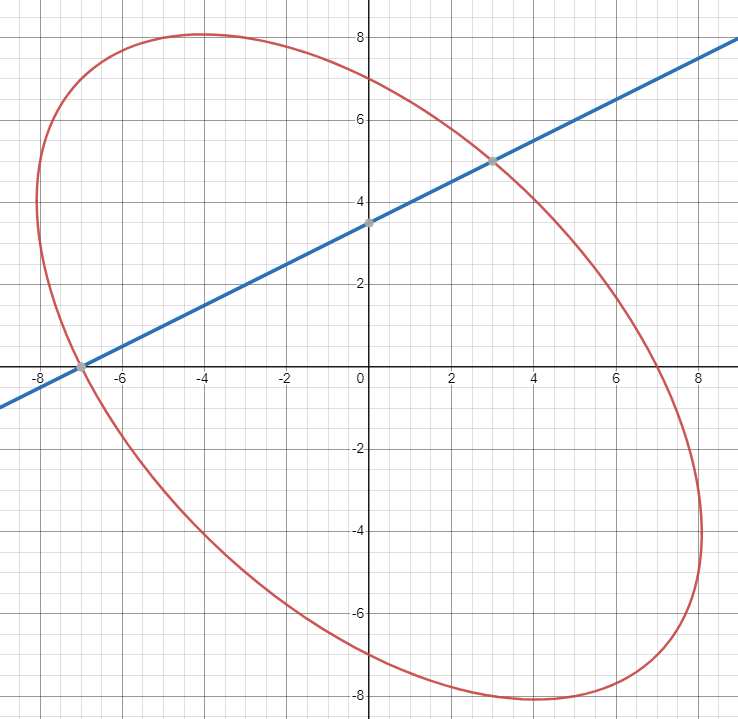
\includegraphics[scale=0.5]{graphing-line-ellipse.png}
\end{center}
\item A line is given by the slope-intercept form
\begin{equation*}
y = -\frac{1}{4}x - 3.
\end{equation*}
\begin{enumerate}
\item Find the slope of the line and the $y$-intercept of the line.
\item Put the equation in standard form and find the $x$-intercept of the line.
\item Find the point on the line with $x$-coordinate $2024$, then put the equation in point-slope form using this point.
\end{enumerate}
\item A line is given by the standard form
\begin{equation*}
3x + y = -4.
\end{equation*}
\begin{enumerate}
\item Find the $x$-intercept and $y$-intercept of the line.
\item Put the equation in slope-intercept form and find the slope of the line.
\item Find the point on the line for which the sum of the coordinates is $10$, then put the equation in point-slope form using this point.
\end{enumerate}
\item A line passes through the point $(-5,2)$ and has slope $1/2$.
\begin{enumerate}
\item Write down an equation for this line in point-slope form.
\item Find the slope-intercept form and the standard form of the line.
\end{enumerate}
\item A line passes through the points $(-3,4)$ and $(-3,-4)$. Find an equation for this line.
\item A line passes through the points $(-3,3)$ and $(0,-4)$.
\begin{enumerate}
\item Find the slope of the line.
\item For each of the two given points, find the point-slope form of the line using that point.
\item Find the slope-intercept form and the standard form of the line.
\end{enumerate}
As a check of your answers, rearranging either of the point-slope equations from part (b) should give you the same slope-intercept form and standard form.
\item A line with equation $y = mx + b$ passes through the points $(5,7)$ and $(8,-1)$. Find $m$ and $b$.
\item Find the point at which the line with equation $2023x + 2022y = 2021$ intersects the line with equation $2024x + 2023y = 2022$.
\item Let $\ell$ be the line with equation $y = -4x - 2$ and let $P = (-4, 2)$. The point $Q$ on line $\ell$ which is closest to $P$ is the point for which $\overline{PQ}\perp\ell$. As such, if $\ell'$ is the line through $P$ perpendicular to line $\ell$, then $Q$ is the intersection of $\ell$ and $\ell'$.
\begin{enumerate}
\item Find the slope of $\ell'$.
\item Find an equation for $\ell'$.
\item Find the coordinates of $Q$.
\end{enumerate}
\end{enumerate}

\subsection{Challenge problems}

\begin{enumerate}[resume]
\item (Perpendicular bisector) Given any two points $A$ and $B$, the \emph{perpendicular bisector} of segment $\overline{AB}$ is the line passing through the midpoint of $\overline{AB}$ which is perpendicular to $\overline{AB}$.
\begin{enumerate}
\item Suppose $B = (14,0)$ and $C = (5,12)$. Find an equation for the perpendicular bisector of segment $\overline{BC}$.
\item Let $P = (x,y)$ be a point in the plane for which $BP = PC$. Find a linear equation relating $x$ and $y$.
\end{enumerate}
\item (Circumcenter) Given any triangle $ABC$, the perpendicular bisectors of the sides of $ABC$ all pass through a single point $O$, called the \emph{circumcenter} of triangle $ABC$. It is the center of the unique circle passing through all three of $A$, $B$, and $C$ (called the \emph{circumcircle} of $ABC$).
\begin{enumerate}
\item Let $A = (0,0)$, $B = (14,0)$, and $C = (5,12)$. Find the circumcenter of $ABC$.
\item Find the radius of the circumcircle of $ABC$ (i.e. the \emph{circumradius} of $ABC$).
\end{enumerate}
\item (Median and centroid) Given any triangle $ABC$, the \emph{medians} are the lines that pass through one vertex and the midpoint of the side opposite that vertex. For example, the $A$-median is the line that passes through $A$ and the midpoint of side $\overline{BC}$. The three medians of a triangle all pass through a single point $G$, called the \emph{centroid} of triangle $ABC$.
\begin{enumerate}
\item Let $A = (0,0)$, $B = (14,0)$, and $C = (5,12)$. Let $D$, $E$, and $F$ be the midpoints of sides $\overline{BC}$, $\overline{CA}$, and $\overline{AB}$, respectively. Find the coordinates of $D$, $E$, and $F$.
\item Find equations for the medians $\overline{AD}$, $\overline{BE}$, and $\overline{CF}$.
\item Find the coordinates of the centroid $G$ of $ABC$. How do they relate to the coordinates of $A$, $B$, and $C$?
\item Compute the ratios $AG/GD$, $BG/GE$, and $CG/GF$.
\end{enumerate}
\item (Altitude and orthocenter) Given any triangle $ABC$, the \emph{altitudes} are the lines that pass through one vertex which are perpendicular to the opposite side. For example, the $A$-altitude is the line that passes through $A$ and is perpendicular to line $\overline{BC}$. The three altitudes of a triangle all pass through a single point $H$, called the \emph{orthocenter} of triangle $ABC$.
\begin{enumerate}
\item Let $A = (0,0)$, $B = (14,0)$, and $C = (5,12)$. Find equations for the altitudes of $ABC$.
\item Find the coordinates of the orthocenter $H$ of $ABC$.
\end{enumerate}
\item Let $A = (1,1)$, $B = (5,2)$, and $C = (-4,3)$. There are three parallelograms in the plane for which $A$, $B$, and $C$ are three of the four vertices. What are the possible coordinates for the fourth vertex?
\end{enumerate}

\newpage
\subsection{Answers}

\begin{enumerate}
\item In your drawing, the origin should be at $(0,0)$, where the coordinate axes intersect. Quadrant I is in the upper right, quadrant II is in the upper left, quadrant III is in the lower left, and quadrant IV is in the lower right.
\item \begin{enumerate}
\item $(3,-1)$
\item $(-3,1)$
\item $(1,3)$
\item $(-3,-1)$
\item $(-1,3)$
\item $(1,1)$
\end{enumerate}
\item \begin{enumerate}
\item $E = (5, 13/2)$; $F = (4, 7/2)$; $G = (-1/2, -2)$; $H = (1/2,1)$
\item The midpoint of $\overline{EG}$ is $(9/4, 9/4)$, which is also the midpoint of $\overline{FH}$.
\end{enumerate}
\item \begin{enumerate}
\item $\boxed{17}$
\item $5 + 13 + 10 + 1 = \boxed{29}$
\end{enumerate}
\item The second and third expressions are valid.
\item \begin{enumerate}
\item The slope is $\boxed{1/4}$, and one of the points on the line is $\boxed{(-1,4)}$.
\item Distributing the right hand side gives us 
\begin{equation*}
y - 4 = \frac{1}{4}x + \frac{1}{4}.
\end{equation*}
Adding 4 to both sides gives us the slope-intercept form
\begin{equation*}
\boxed{y = \frac{1}{4}x + \frac{17}{4}}.
\end{equation*}
The $y$-intercept is $\boxed{(0, 17/4)}$.
\item Subtracting $y$ from both sides, then subtracting $17/4$ from both sides,
\begin{equation*}
\frac{1}{4}x - y = -\frac{17}{4}.
\end{equation*}
To clear denominators, we multiply both sides by $4$ to get the standard form 
\begin{equation*}
\boxed{x - 4y = -17}.
\end{equation*}
When $y = 0$, we have $x = -17$, so the $x$-intercept is $\boxed{(-17, 0)}$.
\end{enumerate}
\item \begin{enumerate}
\item The blue line passes through $(0, 3.5)$, which only satisfies the equation $\boxed{x - 2y = -7}$.
\item The first and last equation describe lines, so the answer cannot be those. Of the remaining two equations, the point $(7,0)$ on the red curve only satisfies $\boxed{x^2 + xy + y^2 = 49}$.
\end{enumerate}
\item \begin{enumerate}
\item The slope is $\boxed{-1/4}$ and the $y$-intercept is $\boxed{(0,-3)}$.
\item To get standard form, we start by moving all of the variables to one side so that $x$ has a positive coefficient and moving all of the constants to the other. Adding $\frac{1}{4}x$ to both sides gives us 
\begin{equation*}
\frac{1}{4}x + y = -3.
\end{equation*}
Multiplying both sides by $4$ gives the standard form 
\begin{equation*}
\boxed{x + 4y = -12}.
\end{equation*}
To get the $x$-intercept, we plug in $y = 0$ to get $x = -12$, so the $x$-intercept is $\boxed{(-12,0)}$.
\item Substituting $x = 2024$ into the slope-intercept form given to us,
\begin{equation*}
y = \left(-\frac{1}{4}\right)\cdot 2024 - 3 = -509.
\end{equation*}
The point-slope form with slope $-1/4$ and point $(2024, -509)$ is
\begin{equation*}
\boxed{y + 509 = -\frac{1}{4}(x - 2024)}.
\end{equation*}
\end{enumerate}
\item \begin{enumerate}
\item Letting $x = 0$, the $y$-intercept is $\boxed{(0, -4)}$.\par
Letting $y = 0$, the $x$-intercept is $\boxed{(-4/3, 0)}$.
\item Solving for $y$ in terms of $x$, the slope-intercept form is 
\begin{equation*}
\boxed{y = -3x - 4}.
\end{equation*}
The slope of the line is $\boxed{-3}$.
\item We want the point $(x,y)$ to lie on the line, i.e. to satisfy $3x + y = -4$, and to have sum of coordinates 10, i.e. $x + y = 10$. Solving the system of equations, $(x,y) = \boxed{(-7,17)}$. The desired point-slope form is then
\begin{equation*}
\boxed{y - 17 = -3(x + 7)}.
\end{equation*}
\end{enumerate}
\item \begin{enumerate}
\item $y - 2 = \frac{1}{2}(x + 5)$
\item Slope-intercept form: $y = \frac{1}{2}x + \frac{9}{2}$\par
Standard form: $x - 2y = -9$
\end{enumerate}
\item The line through the two points is the vertical line $\boxed{x = -3}$.
\item \begin{enumerate}
\item $\dfrac{3 - (-4)}{(-3) - 0} = \boxed{-\frac{7}{3}}$
\item Using $(-3,3)$, we get $\boxed{y - 3 = -\frac{7}{3}(x + 3)}$.\par 
Using $(0, -4)$, we get $\boxed{y + 4 = -\frac{7}{3}(x - 0)}$.
\item Slope-intercept form: $\boxed{y = -\frac{7}{3}x - 4}$\par 
Standard form: $\boxed{7x + 3y = -12}$
\end{enumerate}
\item Substituting the two given points, we get the system of equations
\begin{equation*}
5m + b = 7\qquad\text{and}\qquad 8m + b = -1.
\end{equation*}
Solving yields $\boxed{(m,b) = \left(-\frac{8}{3}, \frac{61}{3}\right)}$.
\item The point of intersection is given by the solution to the system of equations
\begin{align*}
2023x + 2022y &= 2021, \tag{1} \\
2024x + 2023y &= 2022. \tag{2}
\end{align*}
Taking the difference of equations $(2) - (1)$ gives us 
\begin{equation*}
x + y = 1 \tag{3}.
\end{equation*}
Then, $(1) - 2022\cdot (3)$ gives us $x = -1$. Substituting back into $(3)$ gives us $y = 2$, so the point of intersection is $\boxed{(-1,2)}$.
\item \begin{enumerate}
\item Given a line with slope $m\neq 0$, the slope of any line perpendicular to it is given by $-1/m$. Applying this formula with $m = -4$, the slope of $\ell$, tells us the slope of $\ell'$ must be $\boxed{1/4}$.
\item Using point-slope form, since $\ell'$ passes through $P$, one equation for $\ell'$ is 
\begin{equation*}
\boxed{y - 2 = \frac{1}{4}(x + 4)}.
\end{equation*}
\item Solving the system of equations
\begin{equation*}
y = -4x - 2\qquad\text{and}\qquad y - 2 = \frac{1}{4}(x + 4),
\end{equation*}
we find that $Q = \boxed{(-20/17, 46/17)}$.
\end{enumerate}
\item \begin{enumerate}
\item The midpoint of $\overline{BC}$ is $(\frac{14 + 5}{2}, \frac{0 + 12}{2}) = (19/2, 6)$ and the slope is $\frac{0 - 12}{14 - 5} = -4/3$. Thus the slope of the perpendicular bisector is $3/4$, so an equation for it is 
\begin{equation*}
\boxed{y - 6 = \frac{3}{4}\left(x - \frac{19}{2}\right)}.
\end{equation*}
\item Using the distance formula, $BP = PC$ becomes
\begin{align*}
\sqrt{(x - 5)^2 + (y - 12)^2} &= \sqrt{(x - 14)^2 + y^2}, \\
(x - 5)^2 + (y - 12)^2 &= (x - 14)^2 + y^2, \\
x^2 - 10x + 25 + y^2 - 24y + 144 &= x^2 - 28x + 196 + y^2, \\
18x - 24y &= 27.
\end{align*}
Dividing by $3$ gives us the standard form equation $\boxed{6x - 8y = 9}$.\par 
\emph{Remark: The equations found in parts (a) and (b) are equivalent, which tells us that any point which is equidistant from $B$ and $C$ lies on the perpendicular bisector of $\overline{BC}$. Going in the other direction, one can show that every point on the perpendicular bisector of $\overline{BC}$ is equidistant from $B$ and $C$.}
\end{enumerate}
\item \begin{enumerate}
\item To get the circumcenter, we intersect two of the three perpendicular bisectors (we can use the third one to check our work). We found one of the perpendicular bisectors in the previous problem: the perpendicular bisector of $\overline{BC}$ is given by 
\begin{equation*}
y - 6 = \frac{3}{4}\left(x - \frac{19}{2}\right).
\end{equation*}
The perpendicular bisector of $\overline{AB}$ is the vertical line $x = 7$, so at the circumcenter, 
\begin{equation*}
y - 6 = \frac{3}{4}\left(7 - \frac{19}{2}\right) = -\frac{15}{8}.
\end{equation*}
Hence $y = 33/8$ and the circumcenter is $O = \boxed{(7, 33/8)}$.
\item The circumradius is the distance from $O$ to any of $A$, $B$, or $C$. Using $A$,
\begin{equation*}
OA = \sqrt{7^2 + \left(\frac{33}{8}\right)^2} = \boxed{\frac{65}{8}}.
\end{equation*}
\end{enumerate}
\item \begin{enumerate}
\item $D = (19/2, 6)$; $E = (5/2, 6)$; $F = (7,0)$
\item $AD$: $y = \frac{12}{19}x$\par
$BE$: $y = -\frac{12}{23}(x - 14)$\par 
$CF$: $y = -6(x - 7)$
\item $G = (19/3, 4)$; the $x$-coordinate of $G$ is the average of the $x$-coordinates of $A$, $B$, and $C$, and a similar statement holds for the $y$-coordinates.
\item $AG/GD = BG/GE = CG/GF = 2$
\end{enumerate}
\item \begin{enumerate}
\item $A$-altitude: $y = \frac{3}{4}x$\par 
$B$-altitude: $y = -\frac{5}{12}(x - 14)$\par 
$C$-altitude: $x = 5$
\item $(5, 15/4)$
\end{enumerate}
\item Each possible fourth vertex $D$ comes from picking two of the three points $A$, $B$, and $C$ to be opposite each other, and then $D$ will be opposite the third point. We will show how to find $D$ in the case that $A$ and $C$ are opposite each other, i.e. the parallelogram is $ABCD$. We will then provide answers for the case that $A$ and $B$ are opposite each other (so the parallelogram is $ACBD$) and the case that $B$ and $C$ are opposite each other (so the parallelogram is $BACD$).\par 
\emph{Solution 1:} If $ABCD$ is a parallelogram, then $\overline{AB}\parallel\overline{CD}$, so $\overline{AB}$ and $\overline{CD}$ have the same slope. The slope of $\overline{AB}$ is $\frac{1 - 2}{1 - 5} = \frac{1}{4}$, so letting $D = (x,y)$,
\begin{equation*}
\frac{y - 3}{x + 4} = \frac{1}{4}.
\end{equation*}
Multiplying both sides by $4(x + 4)$ (i.e. cross multiplying) turns this into the linear equation $4y - 12 = x + 4$. To get another equation, $\overline{BC}\parallel\overline{AD}$, so $\overline{BC}$ and $\overline{AD}$ have the same slope. The slope of $\overline{BC}$ is $\frac{2 - 3}{5 - (-4)} = -\frac{1}{9}$, so 
\begin{equation*}
\frac{y - 1}{x - 1} = -\frac{1}{9}.
\end{equation*}
Cross multiplying gives us $9y - 9 = 1 - x$. We now have two linear equations for the variables $x$ and $y$, and solving the resulting system of equations gives us $(x,y) = \boxed{(-8,2)}$. By similar reasoning, the point which makes $ACBD$ a parallelogram is $D = \boxed{(10,0)}$, and the point which makes $BACD$ a parallelogram is $D = \boxed{(0,4)}$.\par 
\emph{Solution 2:} A geometry theorem alluded to in Problem 3 states that a quadrilateral $WXYZ$ is a parallelogram if and only if the midpoints of $\overline{WY}$ and $\overline{XZ}$ coincide. Thus for $ABCD$ to be a parallelogram with $D = (x,y)$, we need
\begin{align*}
\text{midpoint of }\overline{AC} &= \text{midpoint of }\overline{BD}, \\
\left(\frac{1 + (-4)}{2}, \frac{1 + 3}{2}\right) &= \left(\frac{5 + x}{2}, \frac{2 + y}{2}\right).
\end{align*}
Matching the first coordinate gives $x = -8$, and matching the second coordinate gives $y = 2$, so $D = \boxed{(-8,2)}$. Similarly, $ACBD$ is a parallelogram when $D = \boxed{(10,0)}$, and $BACD$ is a parallelogram when $D = \boxed{(0,4)}$.
\end{enumerate}